\chapter{O Sistema de Tipos Proposto}\label{capmptc}

\section{Introdu\c{c}\~ao}

No cap\'itulo \ref{sobrecarga} foram apresentados as principais caracter\'isticas da abordagem de Haskell para sobrecarga
e seus principais problemas. Neste cap\'itulo \'e apresentada a defini\c{c}\~ao formal do sistema de tipos proposto 
neste trabalho que visa solucionar, de maneira simples, o principal problema relacionado a ado\c{c}\~ao de tipos com
m\'ultiplos par\^ametros, a saber, ambiguidade de express\~oes que usam nomes sobrecarregados introduzidos em classes 
com m\'ultiplos par\^ametros.

Este cap\'itulo \'e organizado da seguinte maneira. Primeiramente \'e formalizada a sintaxe da linguagem n\'ucleo
considerada. Na se\c{c}\~ao \ref{substituicao}, s\~ao apresentadas algumas propriedades de substitui\c{c}\~oes, a
se\c{c}\~ao \ref{contextos} discorre sobre contextos de tipos e a se\c{c}\~ao \ref{preordem} sobre ordens parciais
sobre tipos e substitui\c{c}\~oes, e \'e apresentado e formalizado um algoritmo capaz de calcular a 
\emph{menor generaliza\c{c}\~ao comum} de um conjunto de tipos \cite{Camarao99a}. A se\c{c}\~ao \ref{sat} 
apresentar\'a detalhes sobre o algoritmo para satisfazibilidade de restri\c{c}\~oes. Finalmente, a se\c{c}\~ao 
\ref{sistema} apresenta o sistema de tipos proposto, seu algoritmo de infer\^encia, detalhes de implementa\c{c}\~ao de
um \emph{front-end} para um compilador Haskell que o utiliza e suas propriedades de tipagem principal e tipo principal.  

\section {Sintaxe}\label{sintaxe}

\subsection{Termos}

A sintaxe dos termos da linguagem n\'ucleo consiste basicamente de \emph{core-ML} \cite{Milner79, Damas82}, mas
chamaremos esta linguagem de \emph{core-Haskell} para enfatizar a exist\^encia de um contexto global que possui todas 
as defini\c{c}\~oes de classes e inst\^ancias (maiores detalhes na se\c{c}\~ao \ref{contextos}). 

Os termos da linguagem s\~ao definidos pela seguinte gram\'atica:

\begin{figure}[h]
	\begin{tabular}{lcll}
		Vari\'aveis de termos (s\'imbolos) & $x\in\text{\textbf{X}}$ &  &\\
		Express\~oes                       & $e\in\text{\textbf{E}}$ & $::=$ & $x$ $|$ $\lambda x.\,e$ $|$ 
		                                                                     $e\,e^{\prime}$
		                                                                     $|$ \texttt{let} $x = e$ \texttt{in} $e$\\
	\end{tabular}
	\centering
	\caption{Sintaxe Livre de Contexto da Linguagem \emph{Core-Haskell}.}
	\label{kernelsyn}
\end{figure}

\subsection{Sintaxe de Tipos e Kinds}

Tipos e \emph{kinds} s\~ao expressos utilizando a seguinte gram\'atica:

\begin{figure}[h]

\[ \begin{array}[c]{llll}
\text{{\small Kind}} & k\,\in\text{\textbf{K}}   & ::= \star \mid k\, \rightarrow k^{\prime} \\
\text{Express\~ao de Tipo Simples} & \mu\in\text{\textbf{T}} & ::= \alpha \mid T \mid 
                                                       \mu_1\:\mu_2 \\
\text{Tipo Simples}      & \tau & \equiv \mu \\
\text{Restri\c{c}\~ao}       & \delta\in(\text{\textbf{C}}\times\overline{\text{\textbf{T}}}) & ::= C\:\overline{\mu} \\
\text{Tipos}             & \sigma\in\Sigma & ::= \tau \mid \kappa\Rightarrow \tau \mid \forall \alpha.\,\sigma \\ \\
\text{Nome de Classe}       & C\in\text{\textbf{C}}  & \hspace*{.5cm} \text{Construtor de Tipos} & T \\
\text{Vari\'avel de Tipo} & \alpha,\beta\in\text{\textbf{V}} & \hspace*{.5cm} \text{{Conjunto de Restri\c{c}\~oes}}   & \kappa \in \mathcal{P}(\text{\textbf{C}}\times\overline{\text{\textbf{T}}})\\
\end{array} \]

\caption{Sintaxe livre de contexto de tipos}
\label{Type-syntax}
\end{figure}

Cabe ressaltar que o nome \emph{vari\'avel de tipo} \'e usado por simplicidade. Na verdade, trata-se de vari\'aveis
de express\~oes de tipo.

\subsubsection{Tipos Simples e Kinds}

Um \emph{kind} \'e uma propriedade de express\~oes de tipos simples. O \emph{kind} de vari\'aveis de tipos e o de 
construtores de tipos s\~ao dados, respectivamente, pelas fun\c{c}\~oes 
$\text{kind}_{\text{\textbf{V}}} : \text{\textbf{V}}\rightarrow\text{\textbf{K}}$ e 
$\text{kind}_{\text{\textbf{C}}} : \text{\textbf{C}}\rightarrow\text{\textbf{K}}$. Estas fun\c{c}\~oes induzem fam\'ilias
indexadas por \emph{kind} de vari\'aveis de tipo e de construtores, especificadas da seguinte maneira:
\begin{center}
	\begin{tabular}{ccl}
		$\text{\textbf{V}}^{k}$ & $=$ & $\{\alpha\in\text{\textbf{V}}\,|\,\text{kind}_{\text{\textbf{V}}}(\alpha)=k\}$\\
		$\text{\textbf{C}}^{k}$ & $=$ & $\{C\in\text{\textbf{C}}\,|\,\text{kind}_{\text{\textbf{C}}}(C)=k\}$\\
	\end{tabular}
\end{center}
Utilizamos um \'indice superior $k$ para identificar o \emph{kind} de vari\'aveis de tipo e construtores:
\begin{center}
	\begin{tabular}{ccc}
  		$\alpha^{k}$ & $\in$ & $\text{\textbf{V}}^{k}$ \\
  		$C^{k}$ & $\in$ & $\text{\textbf{C}}^{k}$ \\
  	\end{tabular}
\end{center}

O \emph{kind} de express\~oes de tipo simples \'e dado pela fun\c{c}\~ao parcial 
\emph{kind}$_{\text{\textbf{T}}}$ : \textbf{T}$\rightarrow$ \textit{K}, definida como:
\begin{equation*}
	\text{kind}_{\text{\textbf{T}}}=\left\{
		\begin{array}{ll}
			k & \text{se $\tau=\alpha^{k}$ ou $\tau = C^{k}$}\\
			k & \text{se $\tau=\tau_{1}\,\tau_{2}$, kind$_{\text{\textbf{T}}}(\tau_{1}) = k^{\prime}\rightarrow k$ e 
			      $kind_{\text{\textbf{T}}}(\tau_{2})=k^{\prime}$}
		\end{array}
	\right.
\end{equation*}
Consideraremos somente express\~oes de tipo que forem \emph{bem formadas}, isto \'e, aquelas que tem um \emph{kind} 
definido. Por isso, o conjunto \textbf{T} s\'o ir\'a incluir express\~oes bem formadas. Por defini\c{c}\~ao, o 
\emph{kind} de tipos simples \'e $\star$.

Como usual,  express\~oes de tipo e de \emph{kind} que envolvem o construtor ($\rightarrow$) s\~ao escritas de forma 
infixa:
\begin{center}
	$\mu_{1}\rightarrow\mu_{2}\equiv ((\rightarrow)\,\mu_{1})\,\mu_{2}$\\
	$k_{1}\,\rightarrow\,k_{2}\equiv ((\rightarrow)\,k_{1})\,k_{2}$\\
\end{center}
onde $\mu_{1}$ e $\mu_{2}$ s\~ao duas express\~oes de tipos e $k_{1},\,k_{2}$ duas express\~oes de \emph{kind}.

A nota\c{c}\~ao $[\mu]$ \'e usada para expressar a aplica\c{c}\~ao do construtor de listas (que possui
 \emph{kind} $\star\rightarrow\star$) ao tipo $\mu$:
 \begin{center}
 	$[\mu]\,\equiv\,([\,\,])\,\mu$
 \end{center}
 
 O conjunto de vari\'aveis de tipo de uma express\~ao de tipo simples \'e dado pela fun\c{c}\~ao 
 \emph{tv} : \textbf{T}$\rightarrow\,\mathcal{P}(\text{\textbf{V}})$, definida como:
\begin{equation*}
	tv(\mu) = \left\{
		\begin{array}{ll}
			\alpha          & \text{se } \mu = \alpha\\
			\emptyset       & \text{se } \mu = C \\
			tv(\mu_{1})\, \cup\, tv(\mu_{2})& \text{se } \mu = \mu_{1}\,\mu_{2}
		\end{array} 
	           \right.
\end{equation*}
Esta opera\c{c}\~ao pode ser utilizada para denotar a fam\'ilia de vari\'aveis de um conjunto 
\textbf{J} de express\~oes de tipo:
\begin{center}
   $tv(\text{\textbf{X}})=\bigcup\{tv(\mu)\,|\,\mu\in\text{\textbf{J}}\}$
\end{center}

\subsubsection{Restri\c{c}\~oes de Classe}

Conforme apresentado na se\c{c}\~ao \ref{polhaskell}, tipos polim\'orficos em Haskell podem conter restri\c{c}\~oes
que limitam as poss\'iveis instancia\c{c}\~oes de vari\'aveis quantificadas neste tipo. Uma restri\c{c}\~ao $\delta$
consiste de um par $(C,\overline{\mu})$, onde $C$ \'e um nome de classe e $\overline{\mu}$ uma sequ\^encia 
de tipos simples, cada tipo simples correspondendo ao par\^ametro da classe de mesma ordem na sequ\^encia em 
$(C,\overline{\mu})$ (se $\overline{\mu}=\{\mu_{1},\,...,\,\mu_{n}\}$ ent\~ao $\mu_{1}$ corresponde ao primeiro 
par\^ametro, $\mu_{2}$ ao $2^{o}$ par\^ametro, ..., $\mu_{n}$ ao $n$-\'esimo par\^ametro da classe $C$). Por quest\~ao
de simplicidade, representaremos o par $(C,\overline{\mu})$ como $C\,\,\overline{\mu}$.

O conjunto de vari\'aveis de tipos de uma restri\c{c}\~ao \'e dado pela fun\c{c}\~ao:
\begin{center}
	$tv:(\text{\textbf{C}}\times\overline{\text{\textbf{T}}})\rightarrow\mathcal{P}(\text{\textbf{V}})$
\end{center} 
onde $tv(C\,\,\overline{\mu})=tv(\overline{\mu})$.
A mesma fun\c{c}\~ao pode ser estendida para conjuntos de restri\c{c}\~oes de maneira simples:
\begin{center}
	$tv(\kappa) = \bigcup_{1 \leq i\leq n} tv(\mu_{i})$ para $\kappa=\{C_{1}\,\,\overline{\mu_{1}},...,C_{n}\,\,
	\overline{\mu_{n}}\}$ e $n\geq 0$.
\end{center} 


\subsubsection{Tipos}

Uma express\~ao $\sigma=\forall\overline{\alpha}.\kappa.\tau$ denota um tipo. Se $\kappa=\emptyset$, dizemos que 
este \'e um tipo irrestrito, caso contr\'ario dizemos que \'e restringido. Caso $\overline{\alpha}=\emptyset$, 
dizemos que este \'e um tipo monom\'orfico, caso contr\'ario dizemos que \'e um tipo polim\'orfico. 
Para simplificar a sintaxe, usamos as seguintes abrevia\c{c}\~oes:
\begin{itemize}
	\item $\forall\overline{\alpha}.\tau$, quando $\kappa = \emptyset$;
	\item $\kappa.\tau$, quando $\overline{\alpha}=\emptyset$;
	\item $\tau$, quando $\kappa = \overline{\alpha}=\emptyset$.
\end{itemize} 
O conjunto de vari\'aveis livres de um tipo \'e dado pela fun\c{c}\~ao 
$tv : \Sigma\rightarrow\mathcal{P}(\text{\textbf{V}})$, definida a seguir:
\begin{center}
	$tv(\forall\overline{\alpha}.\kappa.\tau)=(tv(\kappa)\cup\,tv(\tau)) - \overline{\alpha}$
\end{center}
onde $\overline{\alpha}=\{\alpha_{1},\alpha_{2},...,\alpha_{n}\}$.

Novamente, esta fun\c{c}\~ao pode ser estendida para conjuntos de tipos da seguinte maneira:
\begin{center}
   $tv(\text{\textbf{X}})=\bigcup\{tv(\sigma)\,|\,\sigma\in\text{\textbf{X}}\}$
\end{center}

\section{Substitui\c{c}\~oes}\label{substituicao}

Uma substitui\c{c}\~ao $S$ \'e uma fun\c{c}\~ao de tipo para express\~oes de tipo simples. O conjunto de todas as 
substitui\c{c}\~oes \'e denotado por \textbf{S} e a substitui\c{c}\~ao identidade \'e denotada por \textit{id}.

Define-se o dom\'inio de uma substitui\c{c}\~ao $S$, dom($S$), como o conjunto de vari\'aveis 
$\alpha\in\text{\textbf{V}}$ para as quais $S(\alpha)$ \'e distinto de $\alpha$: 
\begin{center}
	dom($S$) = $\{\alpha\,|\,S(\alpha)\neq\alpha\}$
\end{center}

Neste trabalho consideramos apenas substitui\c{c}\~oes para as quais o conjunto dom($S$) \'e finito e que preservam
o $kind$ das vari\'aveis, i.e. $S(\alpha^{k})\in T^{k}$ para qualquer $kind$ $k\in \text{\textbf{K}}$.

Toda substitui\c{c}\~ao $S$ pode ser estendida para um homomorfismo sobre express\~oes de tipo simples usando o operador
$\text{(  )}^{*}$, definido como:
\begin{center}
\begin{tabular}{lcl}
    $S^{*}(\alpha)$ & $=$ & $S(\alpha)$\\
    $S^{*}(C)$ & $=$ & $C$\\
    $S^{*}(\mu_{1}\,\mu_{2})$ & $=$ & $S^{*}(\mu_{1})\,S^{*}(\mu_{2})$\\
\end{tabular}
\end{center}
Para evitar o excesso de nota\c{c}\~ao, escreveremos $S(\mu)$ ao inv\'es de $S^{*}(\mu)$, e $S\mu$ ao
inv\'es de $S(\mu)$. O termo $[\alpha\,\mapsto\,\mu]$ denota a substitui\c{c}\~ao definida como:
\begin{equation*}
    [\alpha\,\mapsto\,\mu](\beta) = \left\{
    									\begin{array}{ll}
    										\mu  & \text{se } \alpha = \beta\\
    										\beta & \text{se } \alpha \neq \beta
    									\end{array}
                                     \right.
\end{equation*}
Uma substitui\c{c}\~ao pode ser especificada por um conjunto de pares $(\alpha\mapsto\mu)$. Para $n\geq 1$ e para
$\alpha_{i}\neq\alpha_{j}$, com $1\leq i < j\leq n$, a nota\c{c}\~ao 
$[\alpha_{1}\mapsto\mu_{1},...,\alpha_{n}\mapsto\mu_{n}]$ denota a substitui\c{c}\~ao $S$ tal que:
\begin{equation*}
    S(\alpha) = \left\{
                   \begin{array}{ll}
                   	   \mu_{i} & \text{se } \alpha = \alpha_{i}\\
                   	   \alpha   & \text{caso contr\'ario}
                   \end{array}
                \right.
\end{equation*}


Substitui\c{c}\~oes podem ser estendidas usando homomorfismos para o dom\'inio de restri\c{c}\~oes ($S\,\delta$), 
conjuntos de restri\c{c}\~oes ($S\,\kappa$) e tipos restringidos ($S(\kappa.\tau)$), i.e. aplicando a substitui\c{c}\~ao
a cada vari\'avel de tipo que aparece como subtermo. A extens\~ao de uma substitui\c{c}\~ao para uma fun\c{c}\~ao de 
conjuntos de tipos para conjuntos de tipos \'e definida como:
\begin{center}
    $S(X)=\bigcup\{S\mu\,|\,\mu\in X\}$
\end{center}
onde $X$ \'e um conjunto de express\~oes de tipos.

Uma substitui\c{c}\~ao tamb\'em pode ser estendida para uma opera\c{c}\~ao sobre tipos polim\'orficos, mas \'e 
necess\'ario cuidado para evitar a captura de vari\'aveis ligadas. A aplica\c{c}\~ao de uma substitui\c{c}\~ao $S$
a um tipo $\sigma$ \'e dita \emph{livre de captura} se $tv(S\sigma)=tv(S(tv(\sigma)))$.

A fun\c{c}\~ao $tv$ \'e estendida para substitui\c{c}\~oes conforme a seguinte defini\c{c}\~ao:
\begin{center}
    $tv(S) = dom(S)\cup\{tv(S(\alpha))\,|\,\alpha\in\,dom(S)\}$
\end{center}

\section{Contextos de Tipos}\label{contextos}

Um contexto de tipos \'e conjunto que cont\'em informa\c{c}\~oes sobre um programa, que podem ser
utilizadas pelas regras do sistema de tipos. Neste trabalho faremos a distin\c{c}\~ao entre 
tr\^es contextos distintos, a saber:
\begin{itemize}
	\item $\Gamma^{s}\subseteq \text{\textbf{X}}\times\text{\textbf{T}}$: Contexto formado pelas suposi\c{c}\~oes de
	      tipos para s\'imbolos sobrecarregados ou n\~ao. Veja explica\c{c}\~ao no item seguinte.
\item $\Gamma^{cls}\subseteq\text{\textbf{C}}\times\overline{\text{\textbf{V}}}\times
       \mathcal{P}(\textbf{C}\times\overline{\text{\textbf{T}}})$:
          Contexto formado pelas restri\c{c}\~oes de classes definidas no programa. Cada classe      
\begin{flushleft}
\verb|           |\texttt{class $\forall\overline{\alpha}.\kappa\,\Rightarrow\,C\overline{\alpha}$ where}\\
\verb|               | $x_{1}::\kappa_{1}\Rightarrow\tau_{1}$\\
\verb|                      |$\vdots$\\
\verb|               |$\,x_{n}::\kappa_{n}\Rightarrow\tau_{n}$
\end{flushleft}
introduz uma \emph{restri\c{c}\~ao de classe} $(C,\overline{\alpha},\kappa)$ em $\Gamma^{cls}$. Por simplicidade,
a tripla $(C,\overline{\alpha},\kappa)$ ser\'a representada como:
$\forall\overline{\alpha}.\kappa\Rightarrow\,C\,\overline{\alpha}$. 

Al\'em desta restri\c{c}\~ao em $\Gamma^{cls}$, esta declara\c{c}\~ao de classe introduz  
suposi\c{c}\~oes de tipos em $\Gamma^{s}$: $x_{i}\,::\,\sigma_{i}$
onde $\sigma_{i}=\forall\overline{\alpha_{i}}.\kappa\cup\kappa_{i}\Rightarrow\tau_{i}$ e
$\overline{\alpha_{i}}=tv(\kappa\cup\kappa_{1}\Rightarrow\tau_{i})$.
 
Adicionalmente, definiremos $\Gamma^{cls}(C)=\forall\overline{\alpha}.\kappa\Rightarrow\,C\,\overline{\alpha}$ e
$\Gamma^{cls}(x_{i})=\sigma_{i}$ ($\Gamma^{cls}(x)$ \'e indefinido se $x$ n\~ao \'e um s\'imbolo sobrecarregado).

	\item $\Gamma^{ins}\subseteq \text{\textbf{C}}\times\overline{\text{\textbf{T}}}\times
	      \mathcal{P}(\textbf{C}\times\overline{\text{\textbf{T}}})$: 
	      Contexto formado pelas restri\c{c}\~oes de inst\^ancias definidas no programa. Cada inst\^ancia:
\begin{flushleft}
\verb|           |\texttt{instance $\kappa\,\Rightarrow\,C\overline{\mu}$ where}\\
\verb|               | $x_{1}\,=\, e_{1}$\\
\verb|                      |$\vdots$\\
\verb|               |$\,x_{n}\,=\,e_{n}$
\end{flushleft}
introduz uma \emph{restri\c{c}\~ao de inst\^ancia} $\forall\overline{\alpha}.\kappa\Rightarrow\,C\,\overline{\mu}$ 
em $\Gamma^{ins}$. Para restri\c{c}\~oes de inst\^ancias, tamb\'em utilizaremos uma nota\c{c}\~ao similar a j\'a
adotada para tipos. Denotaremos por $\Gamma^{ins}(C)$ o conjunto de restri\c{c}\~oes de inst\^ancias definidas para
uma classe $C$.    
\end{itemize}
O contexto de tipos do escopo mais externo de um programa (escopo global),$\Gamma_{o}$, \'e a uni\~ao de cada um
destes contextos, i.e.  $\Gamma_{o} = \Gamma^{s}\cup\Gamma^{cls}\cup\Gamma^{ins}$. 
 
Nas defini\c{c}\~oes anteriores n\~ao foi imposta nenhuma restri\c{c}\~ao sobre as inst\^ancias. Por\'em, consideraremos
que $\Gamma^{ins}$ cont\'em apenas restri\c{c}\~oes de inst\^ancia bem formadas. Antes de introduzirmos a 
defini\c{c}\~ao de inst\^ancias bem formadas na se\c{c}\~ao \ref{wellformedinst}, apresentaremos a defini\c{c}\~ao de
casamento de classes-inst\^ancias.

\subsection{Casamento de Classes-Inst\^ancias}\label{classinstmatching}

A opera\c{c}\~ao de casamento entre restri\c{c}\~oes de classes e inst\^ancias visa encontrar uma substitui\c{c}\~ao $S$
que torne as cabe\c{c}as de uma classe ($C\,\overline{\alpha}$) e de uma inst\^ancia ($C\,\overline{\mu}$) iguais
(i.e. $S(C\,\overline{\alpha})=\,C\,\overline{\mu}$) e um conjunto $\kappa$ de restri\c{c}\~oes de super-classes de $C$.

\begin{figure}[h]
\small{
\[ \begin{array}{c} 
   \fbox{$\Gamma \models^{cls} \delta\:[S,\kappa]$} \\ [.5cm]
   \displaystyle{\frac{\Gamma^{cls}(C) = \kappa \Rightarrow C \overline{\alpha}\:\:\:\:\:\: S(C \overline{\alpha})=C \overline{\mu}}
	                  {\Gamma \models^{cls} C\overline{\mu}\:[S,\kappa]}} 
   \end{array}
\]}
\caption{Casamento de Classes-Inst\^ancias}
\label{figclassinstmatching} 
\end{figure}



\subsection{Inst\^ancias Bem Formadas}\label{wellformedinst}

Informalmente, uma restri\c{c}\~ao de inst\^ancia $\forall\overline{\alpha}.\kappa\Rightarrow\,C\,\overline{\mu}$ 
\'e bem formada em $\Gamma^{ins}$ se as seguintes condi\c{c}\~oes s\~ao verdadeiras:
\begin{itemize}
	\item $tv(\kappa)\subseteq\, tv(C\,\overline{\mu})$
	\item A cabe\c{c}a da inst\^ancia ($C\,\overline{\mu}$) deve casar com a correspondente restri\c{c}\~ao de classe,
	      i.e. $\Gamma \models^{cls} \delta\:[S,\kappa]$ para algum $S$ e algum $\kappa$.	      
	\item O contexto $\kappa$ deve ser bem formado --- i.e., cada restri\c{c}\~ao 
	      $C^{\prime}\overline{\mu}^{\prime}\in S\,\kappa$, onde 
	       $\Gamma \models^{cls} \delta\:[S,\kappa]$, deve ocorrer em
	      $\kappa$, exceto se $C^{\prime}\overline{\mu}^{\prime}$ n\~ao possui vari\'aveis de tipo, o que torna 
	      necess\'aria a exist\^encia de uma declara\c{c}\~ao de uma inst\^ancia que satisfa\c{c}a esta restri\c{c}\~ao. 
\end{itemize}
As condi\c{c}\~oes anteriores s\~ao expressas formalmente pela regra presente na figura 
\ref{figwellformedinst}.

\begin{figure}[h]
\small{
\[ \begin{array}{c} 
    \fbox{$\Gamma \models^{wfi} \kappa\Rightarrow C\:\overline{\mu}$} \\ [.5cm]
    \begin{array}{c}
	  {\displaystyle \frac{\begin{array}{l}
	                        tv(\kappa) \subseteq tv(C\:\overline{\mu}) \\ [.1cm]
					        \Gamma \models^{cls} C\:\overline{\mu}\:[S_{\scriptscriptstyle{C}},\kappa_{\scriptscriptstyle{C}}] \\ [.1cm]
	                        S_{\scriptscriptstyle{C}}\,\kappa_{\scriptscriptstyle{C}} - \kappa_0 \subseteq \kappa\: 
					        \text{ onde } \:
					        \kappa_0 = \{\delta \in S_{\scriptscriptstyle{C}}\,\kappa_{\scriptscriptstyle{C}}\:|\: tv(\delta)=\emptyset \} \\ [.1cm]
					        \text{para cada } C'\:\overline{\mu}' \in \kappa_0, C'\:\overline{\mu}' \in \Gamma^{ins}(C')
					       \end{array}}
		                 {\Gamma \models^{wfi} \kappa\Rightarrow C\:\overline{\mu}}}
	 
    \end{array}
   \end{array}
\] }
\caption{Restri\c{c}\~ao de Inst\^ancia Bem Formada}
\label{figwellformedinst}
\end{figure}

\subsubsection{Exemplos}

Para tornar mais claras as defini\c{c}\~oes anteriores, vamos considerar o seguinte trecho de c\'odigo de exemplo:
\begin{figure}[h]
\begin{center}
\texttt{
\begin{tabular}{l} 
     class $A\:\alpha\:\:$ where $\:\:\ldots$ \vspace{.1cm} \\
     class $B\:\alpha\:\beta\:\:$ where $\:\:\ldots$  \vspace{.1cm}\\ 
     class $C\:\alpha\:\:$ where $\:\:\ldots$  \vspace{.1cm}\\ 
     class $\{A\:\alpha, B\:\alpha\:\beta\:\}\Rightarrow D\:\alpha\:\beta\:\gamma\:\:$ where $\:\:\ldots$ \vspace{.1cm}\\
     instance $A\:\texttt{Int}\:\:$ where $\:\:\ldots$ \vspace{.1cm} \\ 
	 instance $\{B\:\texttt{Int}\:\beta,\:C\:\gamma\:\}\Rightarrow D\:\texttt{Int}\:\beta\:\gamma\:\:$ where $\:\:\ldots$
\end{tabular}
} 
\end{center}
\caption{C\'odigo de Exemplo para a Defini\c{c}\~ao de Inst\^ancias Bem Formadas}
\label{figexwfinst}
\end{figure}

A inst\^ancia para a classe $D$ \'e bem formada no contexto $\Gamma$ que inclui todas as defini\c{c}\~oes presentes
na figura \ref{figexwfinst}, j\'a que: 
1) $tv(\{B\:\texttt{Int}\:\beta,\:C\:\gamma\:\})\subseteq tv(D\:\texttt{Int}\:\beta\:\gamma)$; 
2) $\Gamma \models^{cls} D\:\text{Int}\:\beta\:\gamma\:[S_{\scriptscriptstyle{D}},\kappa_{\scriptscriptstyle{D}}]$, 
onde $S_{\scriptscriptstyle{D}}=[\alpha\mapsto\text{Int}]$ e 
$\kappa_{\scriptscriptstyle{D}}=\{A\:\alpha,\,B\:\alpha\:\beta\}$; 
3) o contexto para esta declara\c{c}\~ao de inst\^ancia inclui a restri\c{c}\~ao $B\:\text{Int}\:\beta$ 
(que corresponde a $B\:\alpha\:\beta \in \kappa_{\scriptscriptstyle{D}}$), mas n\~ao inclui a restri\c{c}\~ao 
$A\:\texttt{Int}$ (correspondente a $A\:\alpha \in \kappa_{\scriptscriptstyle{D}}$), que n\~ao cont\'em 
vari\'aveis de tipo e possui uma declara\c{c}\~ao de inst\^ancia correspondente. Observe que o contexto de uma 
declara\c{c}\~ao de inst\^ancia pode tamb\'em incluir restri\c{c}\~oes que n\~ao ocorrem em sua declara\c{c}\~ao de
classe, como a restri\c{c}\~ao $C\:\gamma$ na inst\^ancia da classe $D$.


\section{Ordens Parciais}\label{preordem}

Esta se\c{c}\~ao define ordens parciais e seus semi-reticulados correspondentes \cite{Davey90} para um conjunto de
express\~oes de tipos simples, substitui\c{c}\~oes e contextos de tipos. Tais defini\c{c}\~oes ser\~ao utilizadas para a
a demonstra\c{c}\~ao das propriedades de Tipo e Tipagem Principal (definidas na se\c{c}\~ao \ref{tipotipagem}) e na
defini\c{c}\~ao de uma fun\c{c}\~ao para computar a menor generaliza\c{c}\~ao comum de um conjunto de tipos ou 
substitui\c{c}\~oes \cite{Camarao99a}.

\subsection{Express\~oes de Tipos Simples}

\subsubsection{Pr\'e-Ordem de Express\~oes de Tipos Simples}

A rela\c{c}\~ao $\preceq_{\text{\textbf{T}}}$ \'e uma pr\'e-ordem sobre o conjunto de tipos simples, definida como:
\begin{center}
   $\mu\preceq_{\text{\textbf{T}}}\mu^{\prime}$ se e somente se $S\mu = S\mu^{\prime}$, para algum $S$.
\end{center} 

Se $\mu\preceq_{\text{\textbf{T}}}\mu^{\prime}$ e $\overline{\alpha}=tv(\mu)$ e 
$\overline{\alpha}^{\prime}=tv(\mu^{\prime})$, dizemos que $\forall\overline{\alpha}^{\prime}.\mu^{\prime}$ \'e mais 
geral do que $\forall\overline{\alpha}.\mu$, ou que \'e uma generaliza\c{c}\~ao de $\forall\overline{\alpha}.\mu$.

\subsubsection{Equival\^encia M\'odulo Renomeamento de Vari\'aveis}

A partir da pr\'e-ordem  $\preceq_{\text{\textbf{T}}}$ podemos definir a rela\c{c}\~ao de equival\^encia 
$\equiv_{\text{\textbf{T}}}$ como:
\begin{center}
	$\mu\equiv_{\text{\textbf{T}}}\mu^{\prime}$ se e somente se  $\mu\preceq_{\text{\textbf{T}}}\mu^{\prime}$ e
	 $\mu^{\prime}\preceq_{\text{\textbf{T}}}\mu$
\end{center}

Se $\mu\equiv_{\text{\textbf{T}}}\mu^{\prime}$, dizemos que $\mu$ \'e equivalente a $\mu^{\prime}$ m\'odulo renomeamento
de vari\'aveis.

\subsubsection{Ordem Parcial de Express\~oes de Tipos Simples}

Seja $T_{\equiv}$ o conjunto de classes de equival\^encia de $\equiv_{\text{\textbf{T}}}$, podemos estender a pr\'e-ordem
$\preceq_{\text{\textbf{T}}}$ para uma ordem parcial sobre $T_{\equiv}$. Denotaremos por $[\mu]_{\equiv}$ a classe de
equival\^encia de uma express\~ao de tipo simples $\mu$ m\'odulo $\equiv_{\text{\textbf{T}}}$ 
($[\mu]_{\equiv}=\{\mu^{\prime}\,|\,\mu\equiv_{\text{\textbf{T}}}\mu^{\prime}\}$) definimos a ordem parcial 
$\leq_{\text{\textbf{T}}}$ como:
\begin{center}
	$[\mu]_{\equiv}\leq_{\text{\textbf{T}}}[\mu^{\prime}]_{\equiv}$ se e somente se 
	$\mu^{\prime}\preceq_{\text{\textbf{T}}}\mu$
\end{center}

O elemento $[\alpha]$, onde $\alpha$ \'e uma vari\'avel de tipo qualquer, possui a propriedade de ser o 
\emph{elemento m\'aximo} (\emph{majorante}) da ordem parcial, i.e. para todo $\mu$, 
$[\mu]\leq_{\text{\textbf{T}}}[\alpha]$.

Como qualquer elemento de uma classe de equival\^encia pode ser usado para representar a classe, omitiremos os colchetes
e o sinal $\equiv$ quando nos referirmos a elementos de $\text{\textbf{T}}_{\equiv}$, escrevendo $\mu$ ao inv\'es de 
$[\mu]_{\equiv}$.

\subsubsection{Semi-Reticulado de Express\~oes de Tipos Simples}\label{rettiposimples}

Dizemos que $[\mu]=[\mu_{1}]\lor[\mu_{2}]$, ou que $\mu=\mu_{1}\lor\mu_{2}$ ($\mu$ \'e o supremo de $\mu_{1}$ e 
$\mu_{2}$), se $\mu$ for mais geral que $\mu_{1}$ e $\mu_{2}$, e se for o elemento menos geral com esta propriedade.

O supremo de um conjunto finito n\~ao-vazio $X\subseteq\text{\textbf{T}}_{\equiv}$ ($\bigvee\,X$), \'e definido 
como:
\begin{equation*}
	\bigvee\,X=\left\{
					\begin{array}{ll}
					   \mu                 & \text{se } X=\{\mu\}\\
					   \mu\lor\mu^{\prime} & \text{se } X=\{\mu\}\cup X^{\prime}
					                         \text{ e }\mu^{\prime}=\bigvee\,X^{\prime} 
					\end{array}
	           \right.
\end{equation*}

A tupla ($\text{\textbf{T}}_{\equiv}$,$\bigvee$,$[\alpha]$) forma um semi-reticulado com as seguintes propriedades
(que ser\~ao provadas posteriormente):
\begin{itemize}
	\item Para todo $\mu_{1},\mu_{2}\in\text{\textbf{T}}_{\equiv}$, existe $\mu=\mu_{1}\lor\mu_{2}$. Isto \'e,  
	      todo par de elementos de $\text{\textbf{T}}_{\equiv}$ possui supremo.
	\item Para todo $X\subseteq\text{\textbf{T}}_{\equiv}$, existe $\bigvee X$, i.e. todo subconjunto de 
	      $\text{\textbf{T}}_{\equiv}$ possui supremo.
	\item Toda cadeia crescente\footnote{Uma cadeia crescente \'e uma sequ\^encia $\{a_{1},a_{2},...,a_{n}\}$ de 
	      elementos de um conjunto parcialmente ordenado ($P$, $\leq$) tais que $a_{1}\,<\,a_{2}\,<\,...\,<\,a_{n}$.} 
	      de ($\text{\textbf{T}}_{\equiv},\leq_{\text{\textbf{T}}}$) \'e finita.
\end{itemize}

Para exemplificar, a figura \ref{reticuladoex} descreve um fragmento do semi-reticulado de express\~oes de tipo simples.
Note que o tipo simples $\alpha\rightarrow\alpha$ \'e o supremo de $\text{Int}\rightarrow\alpha$ e 
$\alpha\rightarrow\,\text{Int}$, enquanto que o tipo simples $\alpha_{1}\,\,\alpha_{2}$. \'e o supremo dos tipos 
simples Int$\rightarrow$ Int e [Int].

\begin{figure}[h]
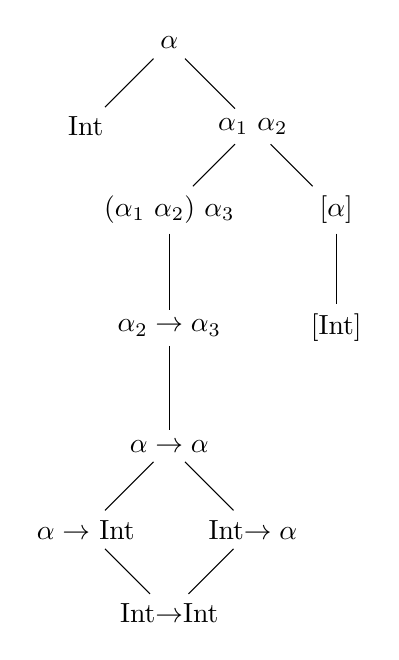
\begin{tikzpicture}[node distance=15mm, element/.style={}]
	\node (alpha)     [element] {$\alpha$} ;
	\node (int)       [element, below left of=alpha] {Int};
	\node (alpha12)   [element, below right of=alpha] {$\alpha_{1}\,\,\alpha_{2}$};
	\node (alpha123)  [element, below left of=alpha12] {$(\alpha_{1}\,\,\alpha_{2})\,\,\alpha_{3}$};
	\node (alphalist) [element, below right of=alpha12] {$[\alpha]$};
	\node (intlist)   [element, below of=alphalist] {[Int]}; 
	\node (alpha23)   [element, below of=alpha123] {$\alpha_{2}\rightarrow\alpha_{3}$};
	\node (alphaa)    [element, below of = alpha23]  {$\alpha\rightarrow\alpha$};
	\node (alphaint)  [element, below left of=alphaa] {$\alpha\rightarrow$ Int};
	\node (intalpha)  [element, below right of=alphaa] {Int$\rightarrow\alpha$};
	\node (intint)    [element, below right of=alphaint] {Int$\rightarrow$Int};	
	\path (alpha)     edge[-] (int)
	      (alpha)     edge[-] (alpha12)
	      (alpha12)   edge[-] (alphalist)
	      (alphalist) edge[-] (intlist)
	      (alpha12)   edge[-] (alpha123)
	      (alpha123)  edge[-] (alpha23)
	      (alpha23)   edge[-] (alphaa)
	      (alphaa)    edge[-] (alphaint)
	      (alphaa)    edge[-] (intalpha)
	      (alphaint)  edge[-] (intint)
	      (intalpha)  edge[-] (intint);         
\end{tikzpicture}
\centering
\caption{Fragmento de Semi-Reticulado de Tipos Simples}
\label{reticuladoex}
\end{figure}

\subsection{Substitui\c{c}\~oes}

\subsubsection{Pr\'e-Ordem de Substitui\c{c}\~oes}

A pr\'e-ordem $\preceq_{\text{\textbf{S}}}$ sobre o conjunto de substitui\c{c}\~oes \textbf{S} \'e definida como:
\begin{center}
	$S_{1}\,\preceq_{\text{\textbf{S}}}\,S_{2}$ se, e somente se existe $S$ tal que $S\circ\,S_{2}=S_{1}$
\end{center}
A pr\'e-ordem $\preceq_{\text{\textbf{S}}}$ induz uma rela\c{c}\~ao de equival\^encia, $\equiv_{\text{\textbf{S}}}$,
definida como:
\begin{center}
	$S_{1}\equiv_{\text{\textbf{S}}}S_{2}$ se, e somente se, $S_{1}\preceq_{\text{\textbf{S}}}S_{2}$ e 
	$S_{2}\preceq_{\text{\textbf{S}}}S_{1}$  
\end{center}

\subsubsection{Ordem Parcial de Substitui\c{c}\~oes}

Tomando $S_{\equiv}$ como o conjunto de classes de equival\^encia de substitui\c{c}\~oes m\'odulo 
$\equiv_{\text{\textbf{S}}}$, e $[S]_{\equiv}$ como a classe de equival\^encia da substitui\c{c}\~ao $S$, podemos definir
a ordem parcial $\leq_{\text{\textbf{S}}}$ sobre $S_{\equiv}$ da seguinte forma:
\begin{center}
	$[S]_{\equiv}\leq_{\text{\textbf{S}}}[S^{\prime}]_{\equiv}$ se, e somente se, 
	$S\preceq_{\text{\textbf{S}}}S^{\prime}$ 
\end{center}

Se $S\preceq_{\text{\textbf{S}}}S^{\prime}$, dizemos que $S^{\prime}$ \'e mais geral (ou uma generaliza\c{c}\~ao de 
$S$), ou ainda que $S$ \'e mais espec\'ifico que $S^{\prime}$ (ou uma especializa\c{c}\~ao de $S^{\prime}$).

O elemento m\'aximo (majorante) desta ordem parcial \'e a substitui\c{c}\~ao identidade (\textit{id}).

Novamente, ser\~ao omitidos os colchetes e o s\'imbolo $\equiv$ quando nos referirmos a elementos de $S_{\equiv}$,
escrevendo $S$ ao inv\'es de $[S]_{\equiv}$.

\subsubsection{Semi-Reticulado de Substitui\c{c}\~oes}

Da mesma maneira que definimos o semi-reticulado dos tipos simples, podemos definir o semi-reticulado de 
substitui\c{c}\~oes ($S_{\equiv}$,$\bigvee$,$id$), que tamb\'em possui as mesmas propriedades citadas na se\c{c}\~ao 
\ref{rettiposimples}. 

A pr\'oxima se\c{c}\~ao apresentar\'a o algoritmo para calcular o supremo (menor generaliza\c{c}\~ao comum) de tipos e
substitui\c{c}\~oes.

\subsection{Tipos}

Em sistemas de tipos com suporte a polimorfismo param\'etrico, a ordena\c{c}\~ao de tipos \'e tal que 
$\forall\alpha.\sigma\leq_{\sigma}[\overline{\alpha}\mapsto\overline{\mu}]\sigma$, para todos os tipos simples $\mu$. 
Por\'em, quando consideramos tipos restringidos, devemos levar em conta as restri\c{c}\~oes presentes nestes tipos 
\cite{Faxen03, Camarao99a}. 

\subsubsection{Ordem Parcial de Tipos}\label{typeinstance}

Seja $\Sigma$ o conjunto de todos os tipos. Podemos definir a ordem parcial $\leq_{\Sigma}$ sobre 
$\Sigma$ da seguinte maneira:
\begin{itemize}
	\item[\ ] $\sigma_{1}\leq_{\Sigma}\sigma_{2}$ se, e somente se existe 
	           $[\overline{\alpha}\mapsto\overline{\mu}]$, tal que 
	           $[\overline{\alpha}\mapsto\overline{\mu}]\sigma_{2}=\sigma_{1}$
	\item[\ ] onde $\sigma_{2}=\forall\overline{\alpha^{\prime}}.\kappa_{2}\Rightarrow\tau$ e 
	          $\overline{\alpha}\subseteq\overline{\alpha^{\prime}}$.
\end{itemize}


\subsection{Contextos de Tipos}

\subsubsection{Ordem Parcial de Contextos de Tipos}

A rela\c{c}\~ao $\leq_{\Gamma}$ \'e uma ordem parcial sobre o conjunto de contextos de tipos, definida como:
\begin{center}
	$\Gamma_{1}\leq_{\Gamma}\Gamma_{2}$ se e somente se para toda vari\'avel $x$, temos que 
	$\Gamma_{1}(x)\leq_{\Sigma}\Gamma_{2}(x)$.
\end{center}

\subsection{Tipagens}

Sejam $\sigma$ e $\Gamma$ serem um tipo e um contexto de tipos respectivamente. D\'a-se o nome de \emph{tipagem} ao par
$(\sigma,\Gamma)$.

\subsubsection{Ordem Parcial de Tipagens}\label{typingorder}

A rela\c{c}\~ao $\leq_{\omega}$ \'e uma ordem parcial sobre o conjunto de tipagens, definida como:
\begin{center}
	$(\sigma_{1},\Gamma_{1})\leq_{\omega}(\sigma_{2},\Gamma_{2})$ se e somente se $\Gamma_{1}\leq_{\Gamma}\Gamma_{2}$ e
	 $\sigma_{1}\leq_{\Sigma}\sigma_{2}$.
\end{center}

As defini\c{c}\~oes das ordens parciais de tipos, contextos de tipos e tipagens ser\~ao utilizadas na se\c{c}\~ao 
\ref{tipotipagem} que formaliza as no\c{c}\~oes de tipo e tipagem principal.

\section{Opera\c{c}\~oes de Supremo}\label{lcg}

Nesta se\c{c}\~ao ser\~ao apresentadas as defini\c{c}\~oes de fun\c{c}\~oes que calculam o supremo de tipos simples e
substitui\c{c}\~oes de acordo com as ordens parciais definidas anteriormente. Estas fun\c{c}\~oes ser\~ao utilizadas 
para permitir a defini\c{c}\~ao opcional de classes de tipos, quando o conjunto de inst\^ancias for conhecido 
\emph{a priori}.

\subsection{C\'alculo do Supremo de Tipos Simples}

A fun\c{c}\~ao que calcula o supremo de dois tipos simples \'e chamada lcg (menor generaliza\c{c}\~ao comum\footnote{
do ingl\^es:\emph{ \textbf{l}east \textbf{c}ommon \textbf{g}eneralization}.}) e sua defini\c{c}\~ao \'e apresentada 
na figura \ref{lcg}.
\begin{figure}[h]
\begin{equation*}
	\begin{array}{rcl}
	\text{lcg}(\mu_{1},\mu_2) & = &\,\, \mu\,\,\text{ onde }(\mu,S_{1},S_{2},V) = \text{lcg}^{\prime}(\mu_{1},\mu_{2}, id, id, tv(\mu_{1})\cup\,tv(\mu_{2}))\\
	                                               & &\\	
	\text{lcg}^{\prime}(T,\mu,S_{1},S_{2},V) & = & \left\{
													  \begin{array}{ll}
													  	(T,S_{1},S_{2},V) & \text{se } \mu = T\\
													  	\text{gen}(T,\mu, S_{1}, S_{2}, V) & \text{caso contr\'ario}
													  \end{array}
	                                               \right.\\
	                                               & &\\
    \text{lcg}^{\prime}(\mu_{1}\,\mu_{2},\mu^{\prime}_{1}\,
           \mu^{\prime}_{2}, S_{1}, S_{2}, V) & = & \left\{
           	                                          \begin{array}{ll}
           	                                          	(\mu\,\mu^{\prime}, S, S^{\prime}, V_{2}) & \text{se }
           	                                          	   kind_{\text{\textbf{T}}}(\mu_{1}) = 
           	                                          	   kind_{\text{\textbf{T}}}(\mu_{2}), \\ 
           	                                          	   & (\mu, S^{\prime}_{1}, S^{\prime}_{2}, V_{1}) =
           	                                          	      \text{lcg}^{\prime}(\mu_{1},\mu^{\prime}_{1}, S_{1},
           	                                          	                          S_{2}, V),\\
           	                                          	   & (\mu^{\prime}, S, S^{\prime}, V_{2}) = 
           	                                          	      \text{lcg}^{\prime}(\mu_{2},\mu^{\prime_{2}}, 
           	                                          	       S^{\prime}_{1}, S^{\prime}_{2}, V_{1})\\
           	                                          	\text{gen}(\mu_{1}\,\mu_{2},\mu^{\prime}_{1}\,\mu^{\prime}_{2},
           	                                          	           S_{1}, S_{2}, V) & \text{caso contr\'ario}
           	                                          \end{array}
                                                    \right. \\
    \text{em todos os outros casos:} &   &\\
    \text{lcg}^{\prime}(\mu_{1},\mu_{2},S_{1},S_{2},V) & = & \text{gen}(\mu_{1},\mu_{2},S_{1},S_{2},V)     
	\end{array}
\end{equation*}
\centering
\caption{Defini\c{c}\~ao da fun\c{c}\~ao lcg}
\label{lcg}
\end{figure}
A fun\c{c}\~ao lcg utiliza a fun\c{c}\~ao auxiliar gen, definida na figura \ref{gen}.
\begin{figure}[h]
\begin{equation*}
	\text{gen}(\mu_{1},\mu_{2},S_{1},S_{2},V) = \left\{
							\begin{array}{l}
							    (\alpha, S_{1}, S_{2}, V)\,\,\text{se }S_{1}(\alpha) = \mu_{1}, 
							                                  S_{2}(\alpha) = \mu_{2}
							                                  \text{ para algum }\alpha\\
							    (\alpha^{\prime}, S^{\prime}_{1}\circ\,S_{1}, S^{\prime}_{2}\circ\,S_{2}, 
							     V\cup\{\alpha^{\prime}\}),\text{ caso contr\'ario,}\\
           	                                          	    \text{onde: }\alpha^{\prime}\not\in V, 
           	                                          	      S^{\prime}_{1}=[\alpha^{\prime}\mapsto\mu_{1}], S^{\prime}_{2}=[\alpha^{\prime}\mapsto\mu_{2}]
							     
							     
							\end{array}
	                                            \right.
\end{equation*}
\centering
\caption{Defini\c{c}\~ao dda fun\c{c}\~ao gen}
\label{gen}
\end{figure}
Esta fun\c{c}\~ao \'e usada para definir a vari\'avel que representar\'a, no tipo resultado da opera\c{c}\~ao, dois
subtermos correspondentes e n\~ao unific\'aveis dos tipos a partir dos quais se est\'a computando o supremo. Ela 
garante que uma mesma vari\'avel seja usada para representar os mesmos subtermos correspondentes. O par\^ametro $V$
representa o conjunto de vari\'aveis ainda n\~ao utilizadas.

\subsection{C\'alculo do Supremo de Substitui\c{c}\~oes}

O supremo de duas substitui\c{c}\~oes \'e calculado pela fun\c{c}\~ao lcgs, definida como:
\begin{equation*}
	\begin{array}{rcl}
		\text{lcgs}(S_{1},S_{2}) & = & S, \text{ onde},\\
		V                        & = & tv(S_{1})\cup tv(S_{2})\\
		(S, S^{\prime},S^{\prime\prime}) & = & \text{lcgs}^{\prime}(\text{dom}(S_{1})\cup\text{dom}(S_{2}),id,id,id)\\
		\text{lcgs}^{\prime}(\emptyset,S,S_{A},S_{B}) & = & S\\
		\text{lcgs}^{\prime}(\alpha,S^{\prime}_{A},S^{\prime}_{B}, V^{\prime}) & = & 
		    \text{lcgs}^{\prime}(S_{1}(\alpha),S_{2}(\alpha),S_{A},S_{B},V)\\
		\text{lcgs}^{\prime}(\{\alpha\}\cup V,S,S_{A},S_{B}) & = &
		    \text{lcgs}^{\prime}(V,[\alpha\mapsto\mu]\circ S, S^{\prime}_{A}, S^{\prime}_{B})\text{ se } V\neq\emptyset
	\end{array}
\end{equation*}

\section{Satisfazibilidade de Restri\c{c}\~oes}\label{sat}

O conjunto de restri\c{c}\~oes $\kappa$ em um tipo $\sigma=\forall\overline{\alpha}.\kappa\Rightarrow\tau$ restringe 
o conjunto de tipos para os quais $\sigma$ pode ser instanciado em um dado contexto $\Gamma$, conforme existam 
suposi\c{c}\~oes em $\Gamma$ que satisfa\c{c}am $\kappa$. Usaremos a nota\c{c}\~ao 
$\Gamma\models^{sat}\kappa[S]$ para representar o fato que o conjunto de restri\c{c}\~oes $\kappa$ \'e satisfeito em 
um contexto $\Gamma$ pela substitui\c{c}\~ao $S$. Definiremos a rela\c{c}\~ao de satisfazibilidade 
gradualmente nesta se\c{c}\~ao, primeiramente para uma restri\c{c}\~ao e depois para conjuntos de restri\c{c}\~oes.

\subsection{Satisfazibilidade de uma Restri\c{c}\~ao}\label{satone}

A restri\c{c}\~ao $C\,\overline{\mu}$ representa um requerimento sobre um contexto. Sua presen\c{c}a no tipo de uma
express\~ao exige a defini\c{c}\~ao de uma inst\^ancia da classe $C$ que a satisfa\c{c}a. Dizemos que uma inst\^ancia 
$\forall\overline{\alpha}.\kappa\Rightarrow\,C\overline{\mu_{1}}$ satistfaz a restri\c{c}\~ao $C\,\overline{\mu}$ se
as seguintes condi\c{c}\~oes s\~ao verdadeiras:
\begin{enumerate} 
	\item Existe uma substitui\c{c}\~ao $S$ tal que $S(C\,\overline{\mu})=S(C\,\overline{\mu_{1}})$.
	\item Existe uma substitui\c{c}\~ao $S^{\prime}$ que satifaz o conjunto de restri\c{c}\~oes $\kappa$, 
	      introduzido pela inst\^ancia $\forall\overline{\alpha}.\kappa\Rightarrow\,C\overline{\mu_{1}}$.
\end{enumerate}
Sendo as duas condi\c{c}\~oes anteriores verdadeiras, temos que substitui\c{c}\~ao
\begin{center} 
	$S_{0}=(S^{\prime}\circ\,S)|_{tv(C\,\overline{\mu})}$ 
\end{center}
satisfaz a restri\c{c}\~ao $C\,\overline{\mu}$ no contexto $\Gamma$. A opera\c{c}\~ao $S_{1}|_{V}$ representa,
informalmente,  a restri\c{c}\~ao do dom\'inio de uma substitui\c{c}\~ao $S_{1}$ sobre um conjunto de vari\'aveis $V$. 
A defini\c{c}\~ao formal desta opera\c{c}\~ao \'e:
\begin{center}
	$S_{1}|_{V} =\{[\alpha\mapsto\tau]\,|\,\alpha\in\,dom(S_{1})\cap\,V\land [\alpha\mapsto\tau]\in\,S_{1}\}$
\end{center}

A regra que define a satisfazibilidade de uma restri\c{c}\~ao \'e a regra (SAT$_{1}$), definida como:

\begin{figure}[h]
	\begin{prooftree}
		\AxiomC{$\kappa\Rightarrow\,C\,\overline{\mu_{1}}\in\Gamma^{ins}(C)$}
		\AxiomC{$S(C\,\overline{\mu})=S(C\,\overline{\mu_{1}})$}
		\AxiomC{$\Gamma\models^{sat}\kappa[S^{\prime}]\,\,\,\,\,S_{0}=S^{\prime}\circ\,S|_{tv(C\,\overline{\mu})}$}
		\RightLabel{\small{(SAT$_1$)}}
		\TrinaryInfC{$\Gamma\models^{sat}\{C\,\overline{\mu}\}[S_{0}]$}
	\end{prooftree}
\caption{Regra para Satisfazibilidade de uma Restri\c{c}\~ao}
\label{figsatone}
%\end{Definition}
\end{figure}


\subsection{Satisfazibilidade de um Conjunto de Restri\c{c}\~oes}\label{satset}  

A satisfazibilidade de um conjunto de restri\c{c}\~oes $\kappa=\{C\,\overline{\mu_{1}},...,C\,\overline{\mu_{n}}\}$ \'e 
definida de maneira an\'aloga a satisfazibilidade de uma restri\c{c}\~ao. Dizemos que um conjunto $\kappa$ de 
restri\c{c}\~oes \'e satisfaz\'ivel em um contexto $\Gamma$ se existe uma substitui\c{c}\~ao $S$ tal
que $S$ seja uma solu\c{c}\~ao para todos os elementos de $\kappa$. 

Desta maneira podemos definir indutivamente a satisfazibilidade de um conjunto de restri\c{c}\~oes. 
Temos que um conjunto vazio de restri\c{c}\~oes \'e trivialmente satisfaz\'ivel por qualquer substitui\c{c}\~ao.
Consideraremos que um conjunto $\kappa=\emptyset$ \'e satisfeito pela substitui\c{c}\~ao identidade ($id$), o que 
nos permite definir a regra SAT$_{\emptyset}$ como:

\begin{figure}[h]
	\begin{prooftree}
		\AxiomC{}
		\RightLabel{\small{(SAT$_{\emptyset}$)}}
		\UnaryInfC{$\Gamma\models^{sat}\emptyset\,[id]$}
	\end{prooftree}
	\caption{Regra para Satisfazibilidade de um Conjunto Vazio de Restri\c{c}\~oes}
	\label{figsatzero}
\end{figure}

Todo conjunto de restri\c{c}\~oes $\kappa$, com $|\kappa|\geq 1$ pode ser escrito da seguinte maneira:
\begin{center}
	$\kappa = \{C\,\overline{\mu}\}\cup\kappa^{\prime}$, 
\end{center}
onde $C\,\overline{\mu}\not\in\kappa^{\prime}$. Tal fato, permite-nos deduzir a regra de satisfazibilidade para 
um conjunto n\~ao vazio de restri\c{c}\~oes (SAT$_{many}$):
\begin{figure}[h]
	\begin{prooftree}
		\AxiomC{$\Gamma\models^{sat}\{C\,\overline{\mu}\}[S_{1}]$}
		\AxiomC{$\Gamma\models^{sat}\kappa[S_{2}]$}
		\RightLabel{\small{(SAT$_{many}$)}}
		\BinaryInfC{$\Gamma\models^{sat}\{C\,\overline{\mu}\}\cup\kappa[S_{2}\circ\,S_{1}]$}
	\end{prooftree}
	\caption{Satisfazibilidade de um Conjunto n\~ao Vazio de Restri\c{c}\~oes}
	\label{figsatmany}
\end{figure}

Intuitivamente, a solu\c{c}\~ao para um conjunto $\kappa$ com $n\geq 1$ restri\c{c}\~oes \'e obtida realizando a 
composi\c{c}\~ao das substitui\c{c}\~oes que satisfazem cada uma das restri\c{c}\~oes $\delta\in\kappa$, o que \'e
representado pela regra SAT$_{many}$ na figura \ref{figsatmany}.

O problema de satisfazibilidade de um conjunto de restri\c{c}\~oes $\kappa$ em um contexto $\Gamma$ \'e indecid\'ivel 
\cite{Volpano91}. Em \cite{Camarao04} \'e apresentado um algoritmo incompleto para o problema que tem sido utilizado
com sucesso na implementa\c{c}\~ao de um algoritmo de infer\^encia de tipos baseado no Sistema CT 
\cite{Camarao07, Camarao99a}.

O algoritmo de satisfazibilidade utilizado neste trabalho \'e baseado na proposta de \cite{Camarao04}, por\'em 
as condi\c{c}\~oes que dever\~ao ser impostas para que se garanta a termina\c{c}\~ao da satisfazibilidade ainda 
dever\~ao ser definidas. Na vers\~ao atual do prot\'otipo implementado, adotamos as restri\c{c}\~oes impostas por 
\cite{Sulzmann06a}. 

\section{Defini\c{c}\~ao do Sistema de Tipos}\label{sistema}

Nesta se\c{c}\~ao \'e apresentado um sistema de tipos para Haskell com suporte a classes com m\'ultiplos par\^ametros
sem a necessidade de depend\^encias funcionais ou fam\'ilias de tipos \cite{Camarao09}. 

Antes de apresentarmos as regras do sistema de tipos, definiremos alguns conceitos necess\'arios.
Primeiramente, definiremos a opera\c{c}\~ao de Fechamento de Conjunto de Restri\c{c}\~oes, que ser\'a utilizada na 
defini\c{c}\~ao de tipos bem formados (se\c{c}\~ao \ref{wellformedty}). A se\c{c}\~ao \ref{simpleq} define a 
simplifica\c{c}\~ao e igualdade de tipos.

\subsection{Fechamento de Conjunto de Restri\c{c}\~oes}\label{closure}

O fechamento de conjunto de restri\c{c}\~oes $\kappa$ com respeito a um conjunto de vari\'aveis de tipo $V$, 
$\kappa\clo_{V}$, \'e definido como: 

\begin{figure}[h]
\[ \begin{array}{l} 
        \kappa \res_V = \{ C\:\overline{\mu} \in \kappa \mid tv(\overline{\mu}) \cap V \not= \emptyset \} \\
        \kappa \clo_V = \left\{ \begin{array}{ll} 
             \kappa\res_V & \text{ se $tv(\kappa\res_V) \subseteq V$}\\ 
             \kappa\clo_{tv(\kappa\res_V)} & \text{ caso contr\'ario}
                                 \end{array} \right.  
      \end{array} \]
      \caption{Fechamento de um Conjunto de Restri\c{c}\~oes}
      \label{figclosure}
\end{figure}
Intuitivamente, $\kappa\clo_{V}$ calcula o conjunto de restri\c{c}\~oes que possui vari\'aveis de tipo 
\emph{alcan\c{c}\'aveis} a partir do conjunto de vari\'aveis $V$. Uma vari\'avel de tipo $\alpha$ \'e alcan\c{c}\'avel 
se $\alpha\in V$ ou $\alpha\in tv(\delta)$, para algum $\delta\in\kappa$ que possua alguma vari\'avel $\beta\in V$ ou
$\beta$ est\'a em outra restri\c{c}\~ao que possui uma vari\'avel presente no conjunto $V$. Dizemos que uma vari\'avel
$\gamma$ \'e \emph{inalcan\c{c}\'avel} se $\gamma\in tv(\kappa)-\kappa\clo_{V}$.

Para exemplificar esta defini\c{c}\~ao, considere o seguinte conjunto de restri\c{c}\~oes: 
\begin{center}
	$\kappa=\{$\texttt{F a b}, \texttt{G a c}$\}$
\end{center}
Temos que $\{$\texttt{F a b}, \texttt{G a c}$\}\clo_{\{c\}}=\{$\texttt{F a b, G a c}$\}$. A restri\c{c}\~ao 
\texttt{G a c} est\'a presente no fechamento pois $tv($\texttt{G a c}$)\cap\{c\}\neq\emptyset$.  J\'a a restri\c{c}\~ao
\texttt{F a b} est\'a presente no fechamento porqu\^e possui uma vari\'avel de tipo (\texttt{a}) que est\'a presente em
uma restri\c{c}\~ao que possui uma vari\'avel (\texttt{c}) pertencente ao conjunto $\{$\texttt{c}$\}$.
 
\subsection{Tipos Bem Formados} \label{wellformedty}

Um tipo restringido $\kappa\Rightarrow\tau$ \'e bem formado em um contexto $\Gamma$, 
$\Gamma\models\kappa\Rightarrow\tau$, se $\Gamma\models^{wf}\kappa\Rightarrow\tau[s]$ \'e prov\'avel de acordo 
com a defini\c{c}\~ao da figura \ref{wellform}:

\begin{figure}[h]
\small{
\[ \begin{array}{c}
       \fbox{$\Gamma\models^{wf} \kappa\Rightarrow\tau\:[S]$} \\ \\
       {\displaystyle \frac{\begin{array}{l}
		                   \text{se existe uma \emph{\'unica} substitui\c{c}\~ao $S$ tal que } \Gamma \models^{sat} \kappa_0\:[S]\:
						   \text{ e }\: tv(S\kappa_0)=\emptyset \\ [.1cm]
						   \text{once} 
						        \begin{array}[t]{l}
						        \kappa_0 = (\kappa - \kappa\clo_V)\: \cup\: \{ \delta \in \kappa\:|\: tv(\delta)=\emptyset\} \\ [.1cm]
						        V=tv(\tau)-tv(\Gamma)
                                \end{array}
					       \end{array}}
                          {\Gamma \models^{wf} \kappa\Rightarrow\tau\:[S]}
		}
	\end{array}
\]}		   
	\caption{Defini\c{c}\~ao de Tipo Bem Formado.}
	\label{wellform}
\end{figure}

Informalmente, um tipo $\kappa\Rightarrow\tau$ \'e bem formado se o conjunto de todas as 
restri\c{c}\~oes em $\kappa$ que n\~ao possuem vari\'aveis de tipo ou que possuem vari\'aveis ``inalcan\c{c}\'aveis''
possui uma \'unica solu\c{c}\~ao em $\Gamma$. \'E importante observar que nesta defini\c{c}\~ao consideramos que o
contexto $\Gamma$ possui apenas restri\c{c}\~oes de classes e inst\^ancias bem formadas de acordo com a defini\c{c}\~ao
presente na se\c{c}\~ao \ref{wellformedinst}

\subsection{Simplifica\c{c}\~ao e Igualdade de Tipos}\label{simpleq}

Seja $\kappa\Rightarrow\tau$ um tipo restringido tal que $\Gamma \models^{wf} \kappa\Rightarrow\tau\:[S]$ \'e prov\'avel
para algum $S$, ent\~ao: 
\begin{itemize}
	\item $S\,\tau=\,\tau$
	\item $S\,\kappa$ n\~ao cont\'em vari\'aveis inalcan\c{c}\'aveis, i.e. $S\kappa\,=\,(S\kappa)\clo_{V}$, 
	      onde $V=tv(\tau)- tv(\Gamma)$.
\end{itemize}
Isto ocorre porqu\^e a substitui\c{c}\~ao $S$ \'e a \'unica solu\c{c}\~ao para $\kappa$ em $\Gamma$. Desta maneira, 
temos que o tipo $\kappa\Rightarrow\tau$ pode ser especializado para 
$\kappa^{\prime}\Rightarrow\tau$, onde:
\begin{center}
 $\kappa^{\prime}=S\,\kappa-\{\delta\in\,S\kappa\,|\,tv(\delta)=\emptyset\}$.
\end{center}
D\'a-se o nome de \emph{simplifica\c{c}\~ao} \`a remo\c{c}\~ao de restri\c{c}\~oes satisfeitas 
(uma restri\c{c}\~ao $\delta$ \'e satisfeita se $tv(\delta)=\emptyset$) em $\kappa$. Usaremos a nota\c{c}\~ao
$\Gamma\models\kappa\Rightarrow\tau\gg\kappa^{\prime}\Rightarrow\tau$, para denotar a simplifica\c{c}\~ao de $\kappa$
para $\kappa^{\prime}$.

A opera\c{c}\~ao de simplifica\c{c}\~ao pode ser estendida para tipos. Um tipo $\sigma$ pode ser simplificado para 
$\sigma^{\prime}$ --- $\Gamma\models\sigma\gg\sigma^{\prime}$, 
onde $\sigma=\forall\overline{\alpha}.\kappa\Rightarrow\tau$ e
$\sigma^{\prime}=\forall\overline{\alpha}^{\prime}.\kappa^{\prime}\Rightarrow\tau$ --- se 
$\Gamma\models\kappa\Rightarrow\tau\gg\kappa^{\prime}\Rightarrow\tau$ e 
$\overline{\alpha}^{\prime}=tv(\kappa^{\prime}\Rightarrow\tau)\cap\overline{\alpha}$.

A simplifica\c{c}\~ao de tipos produz tipos iguais em $\Gamma$. Denotamos por 
$\Gamma\models\sigma\equiv\sigma^{\prime}$ a rela\c{c}\~ao de equival\^encia entre tipos que consiste do fecho 
reflexivo, sim\'etrico e transitivo da rela\c{c}\~ao de simplifica\c{c}\~ao de tipos.  

\subsection{O Sistema de Tipos}\label{typerules}

Um sistema de tipos dirigido por sintaxe\footnote{do ingl\^es:\emph{Syntax Directed Type System}} para 
\emph{core-Haskell} \'e apresentado na figura \ref{figtyperules}. As regras s\~ao similares as regras do
sistema de tipos de Hindley-Milner \cite{Milner79}, exceto pelo uso da instancia\c{c}\~ao de tipos restringidos  
(se\c{c}\~ao \ref{typeinstance}) na regra (VAR). Na regra (LET) \'e requerido que um tipo restringido 
seja bem formado ($\Gamma\models\kappa\Rightarrow\tau$), antes que este seja inclu\'ido em $\Gamma$ e na regra (APP)
o tipo da aplica\c{c}\~ao $e\,e^{\prime}$ inclui as restri\c{c}\~oes que ocorrem nos tipos de $e$ e $e^{\prime}$. 

\begin{figure}[h]
\centering{\fbox{$\Gamma \vdash e: \kappa\Rightarrow\tau$}} \vspace{.5cm}
\begin{align}
   \frac{x:\sigma \in \Gamma \:\:\:\:\:\: \Gamma \models \sigma \leq_{\Sigma} \kappa\Rightarrow\tau}
        {\Gamma \vdash x: \kappa\Rightarrow \tau} & \tag{\small{VAR}} \\[.2cm] 
   \frac{\Gamma,x:\tau' \vdash e: \kappa \Rightarrow \tau} 
        {\Gamma \vdash \lambda x.\:e:\,\kappa\Rightarrow \tau' \rightarrow \tau} & \tag{\small{ABS}}\\[.2cm] 
   \frac{\Gamma \vdash e: \kappa \Rightarrow \tau' \rightarrow \tau \:\:\:\:\:\:\:
         \Gamma \vdash e': \kappa' \Rightarrow \tau'}
        {\Gamma \vdash e\:e': \kappa\cup \kappa'\Rightarrow \tau} & \tag{\small{APP}}\\[.2cm] 
   \frac{\Gamma \vdash e\!:\kappa\!\Rightarrow\!\tau \:\:\:\:\:\:\: \Gamma \models \kappa\Rightarrow\tau
         \:\:\:\:\:\:\:
         \Gamma,\,x\!:\!\sigma \vdash e'\!:\kappa'\!\Rightarrow\!\tau'}
        {\Gamma \vdash \text{\texttt{let }}\ x=e\ \text{\texttt{ in }}\ e':\kappa'\Rightarrow\tau'} & \tag{\small{LET}} \\[.2cm]
       \text{onde: }\begin{array}[t]{l}
	                    \sigma = \forall\overline{\alpha}.\kappa\Rightarrow\tau \\ 
                        \overline{\alpha} = tv(\kappa\Rightarrow \tau)-tv(\Gamma) 
					 \end{array} & \notag
\end{align}
\caption{Regras do Sistema de Tipos}
\label{figtyperules}
\end{figure}

Cabe ressaltar que o sistema de tipos apresentado na figura \ref{figtyperules} prov\^e suporte a classes de tipos 
com m\'ultiplos par\^ametros, mas ainda n\~ao permite a declara\c{c}\~ao opcional de classes de tipos.

Na pr\'oxima se\c{c}\~ao ser\~ao apresentadas propriedades importantes do sistema de tipos descrito nesta se\c{c}\~ao.

\subsection{Propriedades do Sistema de Tipos}\label{tipotipagem}

O sistema de tipos possui a importante propriedade de que a derivabilidade de tipos bem formados \'e fechada sobre a 
aplica\c{c}\~ao de substitui\c{c}\~oes (se todas as restri\c{c}\~oes de classe e inst\^ancias s\~ao bem formadas). 
Essa propriedade \'e conhecida como o \emph{lema da substitui\c{c}\~ao}\footnote{do ingl\^es:\emph{Substitution lemma}}
\cite{Mitchell96}.
\begin{itemize}
	\item[\ ] \textbf{Lema 1} (Substitui\c{c}\~ao): \emph{Seja $\Gamma\vdash\,e\,:\kappa\Rightarrow\tau$. Ent\~ao
	          $\Gamma\models\kappa\Rightarrow\tau$ e para todo $S$ tal que $S\Gamma\models\,S(\kappa\Rightarrow\tau)$,
	          n\'os temos que $S\Gamma\vdash\,e\,:\,S(\kappa\Rightarrow\tau)$.}
\end{itemize}

\'E comum dizer que o sistema de tipos ``tem a propriedade de tipo principal'' se, para qualquer par formado por um
contexto de tipos e uma express\~ao da linguagem, ou n\~ao existe tipo deriv\'avel para a express\~ao neste contexto ou
existe um tipo principal para a express\~ao neste contexto \cite{Damas82, Faxen03}. O conceito de tipo principal n\~ao
deve ser confundido com o de \emph{tipagem principal} \cite{Wells02, Trevor96}. Informalmente, temos:
\begin{center}
\begin{tabular}{ll}
	\textbf{Tipo Principal} & \\
	Dado:                   & um termo $e$ e um contexto $\Gamma$.\\
	Existe:                 & um tipo $\sigma$ que representa todos os tipos\\
	                        & poss\'iveis de $e$ em $\Gamma$.\\
	                        & \\
	\textbf{Tipagem Principal} & \\
	Dado:                      & um termo $e$.\\
	Existe:                    & um tipo $\sigma$ e um contexto $\Gamma$ tais que\\
	                           & $\Gamma$ cont\'em as suposi\c{c}\~oes ``m\'inimas''\\
	                           & para tipagem de $e$, e $\sigma$ representa todos os\\
	                           & tipos que podem ser derivados para $e$ em $\Gamma$.	
\end{tabular}
\end{center}

As defini\c{c}\~oes a seguir formalizam os conceitos de tipo e tipagem principal.

\begin{itemize}
	\item[\ ]\textbf{Defini\c{c}\~ao 1} (Tipo Principal). O tipo principal de uma express\~ao $e$ em um contexto 
	         $\Gamma$ \'e o menor limite superior da ordem parcial $\sigma\leq_{\Sigma}\sigma^{\prime}$, definida na se\c{c}\~ao
	         \ref{typeinstance}.
	\item[\ ]\textbf{Defini\c{c}\~ao 2} (Tipagem Principal). A tipagem principal de uma express\~ao $e$ em um 
	contexto mais externo $\Gamma_{o}$ \'e o menor limite superior da ordem parcial (se\c{c}\~ao \ref{typingorder})
	$(\sigma_{1},\Gamma_{1})\leq_{\omega}(\sigma_{2},\Gamma_{2})$ de todas as tipagens $(\sigma,\Gamma)$ tal que
	$\Gamma\vdash\,e:\kappa\Rightarrow\tau$ \'e prov\'avel e $\sigma=\forall\overline{\alpha}.\kappa\Rightarrow\tau$,
	onde $\overline{\alpha}=tv(\kappa\Rightarrow\tau)-tv(\Gamma)$.
\end{itemize}

\section{Infer\^encia de Tipos}\label{inference}

O algoritmo para infer\^encia de tipos \'e apresentado na figura \ref{figtypeinfer} como um sistema de provas dirigidas
por sintaxe\footnote{do ingl\^es: \emph{Syntax-directed Proof System.}} de julgamentos 
$\Gamma \vdash_{\texttt{I}} e: (\kappa\Rightarrow\tau,\,\Gamma^{\prime})$.

\begin{figure}[h]
\centering{\fbox{$\Gamma \vdash_{\texttt{I}} e: (\kappa\Rightarrow\tau,\,\Gamma^{\prime})$}} 
\begin{align}
       \displaystyle \frac{\Gamma(x) = \forall\,\overline{\alpha}.\,\kappa\Rightarrow\tau }
            {\Gamma \vdash_{\texttt{I}} x: \bigl(\kappa\Rightarrow\tau,\: \{x:\Gamma^*(x)\} \bigr)} 
         & \tag{$VAR_{\texttt{I}}$} \\[.6cm]
       \frac{\displaystyle \Gamma \vdash_{\texttt{I}} (e: \kappa\Rightarrow\tau, \Gamma')}
            {\displaystyle \Gamma \ominus x \vdash_{\texttt{I}} \lambda x.\,e: (\kappa\Rightarrow\tau' \rightarrow \tau,\: 
                                                                   \Gamma' \ominus x)} & \tag{$ABS_{\texttt{I}}$} \\[.3cm]
       \text{where: } \tau' = \left\{ \begin{array}{ll}
                          \tau   & \text{ if } x:\tau \in \Gamma'\\
                          \alpha & \text{ otherwise, $\alpha$ fresh}
                       \end{array}\right. & \notag \\[.6cm]
       \frac{\displaystyle \Gamma \vdash_{\texttt{I}} e: (\kappa\Rightarrow\tau, \Gamma_1) \:\:\:\:\:\:\:\:
                           \Gamma \vdash_{\texttt{I}} e': (\kappa'\Rightarrow\tau', \Gamma_2) } 
            {\displaystyle \Gamma \vdash_{\texttt{I}} e\:e': S' S(\kappa \cup \kappa')\Rightarrow S \alpha,\:
                                                   S\Gamma_1\cup S\Gamma_2)} & \tag{$APP_{\texttt{I}}$}\\[.3cm]
       \text{where: }
           \begin{array}[t]{l}
             S = unify(\{\tau = \tau'\rightarrow\alpha\} \cup st(\Gamma_1,\Gamma_2))\\
             S' = wf(S(\kappa \cup \kappa'\Rightarrow \alpha), \Gamma),\: \alpha \text{ fresh}
           \end{array} & \notag \\[.8cm]
       \frac{\displaystyle \Gamma \vdash_{\texttt{I}} e: (\kappa\Rightarrow\tau,\Gamma_1)   \:\:\:\:\:\:\:\:  
                           \Gamma, \{x:\sigma\} \vdash_{\texttt{I}} e': (\kappa'\Rightarrow\tau',\Gamma_2) }
            {\displaystyle \Gamma \vdash_{\texttt{I}} \text{let }\ x=e\ \text{ in }\ e': (S' S\kappa'\Rightarrow S\tau',\: 
                                                                   S\Gamma' \ominus x)} & \tag{$LET_{\texttt{I}}$} \\[.3cm]
       \text{where: }
          \begin{array}[t]{l}
		     S_0 = wf(\kappa\Rightarrow\tau,\Gamma_1) \\
			 \sigma = \forall \overline{\alpha}.\,S_0\kappa\Rightarrow \tau \\
			 \overline{\alpha}=tv(S_0\kappa\Rightarrow \tau)-tv(\Gamma_1) \\
             S = unify(st(\Gamma_1,\Gamma_2))\\
             S' = wf(S(\kappa \cup \kappa'\Rightarrow \tau'),\Gamma)
          \end{array} & \notag
\end{align}
\caption{Algoritmo para Infer\^encia de Tipagens Principais}
\label{figtypeinfer} 
\end{figure}



Seja $\Theta(\Gamma)$ o contexto de tipos mais externo contendo restri\c{c}\~oes de classes, inst\^ancias e o 
tipo principal de cada s\'imbolo sobrecarregado, isto \'e:

  \[ \Theta(\Gamma) =  
        \bigcup_C \Gamma^{cls}(C) \cup
        \bigcup_C \Gamma^{ins}(C) \cup 
        \bigcup_x \Gamma(x)
  \]
onde $C$ representa um nome de classe e $x$ um s\'imbolo sobrecarregado. Note que $\Theta(\Gamma)$ n\~ao \'e igual a 
$\Gamma_{o}$ (definido na se\c{c}\~ao \ref{contextos}), uma vez que $\Theta(\Gamma)$ inclui somente informa\c{c}\~oes
sobre s\'imbolos sobrecarregados e $\Gamma_{o}$ inclui toda a informa\c{c}\~ao de s\'imbolos sobrecarregados ou n\~ao.

Adicionalmente, o algoritmo de infer\^encia utiliza as seguintes nota\c{c}\~oes:

  \[ \begin{array}{l}
       \Gamma(x) = \left\{\begin{array}{ll}
          \kappa\Rightarrow \tau & \text{\small{se $x$ \'e um s\'imbolo sobrecarregado e 
		                                        $\Gamma^{cls}(x)=\forall\,\overline{\alpha}.\,\kappa\Rightarrow\tau$}}\\
		                         & \text{{\small ou $x$ \'e uma vari\'avel de tipo let ou lambda or e $x:\forall\,\overline{\alpha}.\,\kappa\Rightarrow\tau \in \Gamma$}} \\
	                             & \text{{\small \hspace{.3cm} onde as vari\'aveis de tipo de $\kappa\Rightarrow\tau$ 
	                             s\~ao novas vari\'aveis de tipo.}}\\
          \alpha         & \text{\small{caso contr\'ario, onde $\alpha$ \'e uma nova vari\'avel de tipo}}
     \end{array}\right. \\ \\
     \Gamma^*(x) = \Gamma(x) \cup \Theta(\Gamma)\\
     \Gamma \ominus x = \Gamma -\{ x:\sigma \mid \text{$x$ \'e uma vari\'avel de tipo let ou lambda}, \sigma\in \Gamma(x)\}
    \end{array}
  \]

Tamb\'em s\~ao usadas as fun\c{c}\~oes $lb$, $st$, $unify$ e $wf$, onde $unify$ \'e uma fun\c{c}\~ao para unificar dois
tipos; $lb(\Gamma)$ denota o subconjunto de suposic\c{c}\~oes de tipo para vari\'aveis de tipo lambda em $\Gamma$ e
$st(\Gamma,\Gamma^{\prime})$ produz o conjunto de igualdades entre tipos simples de cada vari\'avel lambda presente em
em $\Gamma$ e $\Gamma^{\prime}$ (que devem ser unificadas durante a infer\^encia, j\'a que est\~ao restritas a possuir
tipos monom\'orficos):
 \[ st(\Gamma,\Gamma') = \{ \tau = \tau' \mid 
        x:\tau \in lb(\Gamma),\: x:\tau' \in lb(\Gamma') \} \]

A fun\c{c}\~ao $wf$ \'e utilizada para verificar se um tipo $\kappa\Rightarrow\tau$ \'e bem formado em um contexto
$\Gamma$, de acordo com a defini\c{c}\~ao de $\Gamma\models^{wf}\kappa\Rightarrow\tau$ apresentada na se\c{c}\~ao 
\ref{wellformedty}. A defini\c{c}\~ao da fun\c{c}\~ao $wf$ \'e apresentada na figura \ref{figwffun}.

\begin{figure}[h]
\begin{center}
\parbox{\textwidth}{
   {\begin{tabbing}
      xx\= ix\= ixxxxx\= \kill
      {\textit{wf}}($\kappa\Rightarrow\tau,\Gamma$) = \+ \\
        \textit{let } $\kappa_0 = \kappa - \kappa\clo_{tv(\tau)}\: \cup \: \{ \delta \in \kappa\:|\: tv(\delta)=\emptyset\: \}$ \\
		\textit{in  if $\kappa_0=\emptyset$ then id} \+ \\
        \textit{ else case} $sat$($\kappa_0,\Gamma$) \textit{of} \+\\
                   $(Ambiguous,\_)$\=xx\= \kill
                   $(Unsat,\_)$       \>$\rightarrow$ \textit{"error: $\,\,\,\,\,$unsatisfiability \ldots"}\\ 
                   $(Single,S)$   \>$\rightarrow$ \textit{if $tv(S\kappa_0)=\emptyset$ then $S$}\\ 
				                       \>\> \textit{ else "error: $\,\,\,\,\,$ambiguity \ldots"} \\ 
                    $(Many, \_)$   \>$\rightarrow$ \textit{"error:  $\,\,\,\,\,$ambiguity \ldots"}\-\-\\
   \end{tabbing} }
}
\end{center}
\caption{Fun\c{c}\~ao para determinar se um tipo \'e bem formado}
\label{figwffun}
\end{figure}

A defini\c{c}\~ao de $wf$ usa a fun\c{c}\~ao $sat$($\kappa$,$\Gamma$), definida em \cite{Camarao04, Camarao07}, que 
implementa a rela\c{c}\~ao $\Gamma\models^{sat}\kappa[S]$ (se\c{c}\~ao \ref{sat}) para obter uma solu\c{c}\~ao para o
problema de satisfazibilidade $(\kappa,\Gamma)$, caso esta exista. Mais precisamente, a fun\c{c}\~ao $sat$ um conjunto
de poss\'iveis solu\c{c}\~oes para o problema. Caso n\~ao exista solu\c{c}\~ao ($Unsat$) ou exista mais de uma ($Many$)
uma mensagem de erro \'e retornada indicando a insatisfazibilidade ou ambiguidade de $\kappa$ em $\Gamma$. Se existir
uma \'unica solu\c{c}\~ao para $\kappa$ esta \'e utilizada para especializar este conjunto de restri\c{c}\~oes. Note que
o teste de satisfazibilidade \'e executado em $wf$ apenas quando existem vari\'aveis inalcan\c{c}\'aveis (se\c{c}\~ao
\ref{closure}) em $\kappa$, e que portanto precisam ser resolvidas ou o tipo em quest\~ao ser\'a considerado amb\'iguo.

\section{Conclus\~ao}

Neste cap\'itulo foi apresentado um sistema de tipos para Haskell que permite a defini\c{c}\~ao de classes de tipos
com m\'ultiplos par\^ametros que n\~ao requer extens\~oes como depend\^encias funcionais e fam\'ilias
de tipos para evitar a ocorr\^encia de tipos amb\'iguos. Tal sistema \'e uma solu\c{c}\~ao minimalista para a
a ado\c{c}\~ao de classes com m\'ultiplos par\^ametros em Haskell \cite{Camarao09}, j\'a que n\~ao exige nenhuma
extens\~ao ao sistema de classes de tipos. 
